\documentclass[aspectratio=169]{beamer}
\usepackage[utf8]{inputenc}
\usepackage[T1]{fontenc}
\usepackage{lmodern}
\usepackage{xcolor}
\usepackage{tikz}
\usetikzlibrary{positioning}
\usepackage{pgfplots}
\pgfplotsset{compat=1.18}
\usetheme{Madrid}

\title{Lexical Scanner Using Flex}
\subtitle{Compiladores e Interpretes -- Lexical Analysis}
\author[F. Benavides, M. Gaviria, M. Zamora]{Felipe Benavides \\ Matthew Gaviria Brenes \\ Marvin Zamora Mussio}
\institute[TEC]{Ingenieria en Computadores}
\date{Semestre I -- 2026}

\definecolor{keywordcolor}{RGB}{30,70,150}
\definecolor{identifiercolor}{RGB}{20,120,70}
\definecolor{integercolor}{RGB}{150,80,20}
\definecolor{floatcolor}{RGB}{180,100,20}
\definecolor{stringcolor}{RGB}{120,40,120}
\definecolor{charcolor}{RGB}{150,50,50}
\definecolor{operatorcolor}{RGB}{110,30,150}
\definecolor{delimitercolor}{RGB}{70,70,70}
\definecolor{errorcolor}{RGB}{190,20,20}
\definecolor{errorbackground}{RGB}{255,220,220}

\newcommand{\KW}[1]{\textcolor{keywordcolor}{\textbf{#1}}}
\newcommand{\ID}[1]{\textcolor{identifiercolor}{\textit{#1}}}
\newcommand{\INT}[1]{\colorbox{integercolor!15}{\textcolor{integercolor}{#1}}}
\newcommand{\FLOAT}[1]{\colorbox{floatcolor!15}{\textcolor{floatcolor}{#1}}}
\newcommand{\STR}[1]{\colorbox{stringcolor!12}{\textcolor{stringcolor}{#1}}}
\newcommand{\CHAR}[1]{\colorbox{charcolor!12}{\textcolor{charcolor}{#1}}}
\newcommand{\OP}[1]{\textcolor{operatorcolor}{\textbf{#1}}}
\newcommand{\DELIM}[1]{\textcolor{delimitercolor}{#1}}
\newcommand{\ERR}[1]{\colorbox{errorbackground}{\textcolor{errorcolor}{\textbf{#1}}}}

\begin{document}

\begin{frame}
\titlepage
\end{frame}

\begin{frame}{Lexical Analysis}
\begin{itemize}
\item The scanner is the first phase of the compiler pipeline
\item It reads the input produced by the preprocessing phase
\item Whitespace and comments are ignored
\item The scanner recognizes lexemes and classifies them into token categories
\item Invalid characters are reported as lexical errors
\end{itemize}
\end{frame}

\begin{frame}{Scanner Architecture}
\begin{center}
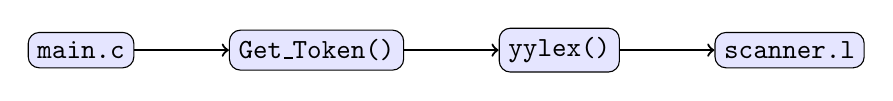
\begin{tikzpicture}[node distance=1.4cm, auto]
\node[draw, rounded corners, fill=blue!10] (main) {\texttt{main.c}};
\node[draw, rounded corners, fill=blue!10, right=1.2cm of main] (get) {\texttt{Get\_Token()}};
\node[draw, rounded corners, fill=blue!10, right=1.2cm of get] (flex) {\texttt{yylex()}};
\node[draw, rounded corners, fill=blue!10, right=1.2cm of flex] (rules) {\texttt{scanner.l}};
\draw[->, thick] (main) -- (get);
\draw[->, thick] (get) -- (flex);
\draw[->, thick] (flex) -- (rules);
\end{tikzpicture}
\end{center}
\par\vspace{0.6cm}
\centering Each call to \texttt{Get\_Token()} requests the next recognized token from the Flex scanner.
\end{frame}

\begin{frame}{Flex}
\begin{itemize}
\item Flex generates a lexical analyzer from regular-expression rules
\item Rules combine patterns with C actions
\item The longest matching rule is selected
\item The generated scanner is compiled together with the C modules
\item The project uses Flex to implement lexical recognition
\end{itemize}
\end{frame}

\begin{frame}{Lexeme Visualization}
\small
\begin{tabular}{ll}
\KW{keyword} & Keyword \\
\ID{identifier} & Identifier \\
\INT{123} & Integer literal \\
\FLOAT{45.67} & Floating-point literal \\
\STR{"text"} & String literal \\
\CHAR{'A'} & Character literal \\
\OP{+} & Operator \\
\DELIM{;} & Delimiter \\
\ERR{@} & Lexical error \\
\end{tabular}
\end{frame}

\begin{frame}[fragile]{Source Entering the Scanner (lines 1--16)}
\tiny
\begin{block}{}
\ttfamily
\obeylines
\KW{int}\hspace*{0.18em}\ID{main}\DELIM{(}\DELIM{)}\hspace*{0.18em}\DELIM{\{}
\hspace*{0.18em}\hspace*{0.18em}\hspace*{0.18em}\hspace*{0.18em}\KW{int}\hspace*{0.18em}\ID{number}\hspace*{0.18em}\OP{=}\hspace*{0.18em}\INT{123}\DELIM{;}
\hspace*{0.18em}\hspace*{0.18em}\hspace*{0.18em}\hspace*{0.18em}\KW{float}\hspace*{0.18em}\ID{value}\hspace*{0.18em}\OP{=}\hspace*{0.18em}\FLOAT{45.67}\DELIM{;}
\hspace*{0.18em}\hspace*{0.18em}\hspace*{0.18em}\hspace*{0.18em}\KW{char}\hspace*{0.18em}\ID{letter}\hspace*{0.18em}\OP{=}\hspace*{0.18em}\CHAR{'A'}\DELIM{;}
\hspace*{0.18em}\hspace*{0.18em}\hspace*{0.18em}\hspace*{0.18em}\KW{const}\hspace*{0.18em}\KW{char}\hspace*{0.18em}\OP{*}\ID{text}\hspace*{0.18em}\OP{=}\hspace*{0.18em}\STR{"Hello\hspace*{0.18em}World"}\DELIM{;}

\hspace*{0.18em}\hspace*{0.18em}\hspace*{0.18em}\hspace*{0.18em}\ID{number}\OP{++}\DELIM{;}
\hspace*{0.18em}\hspace*{0.18em}\hspace*{0.18em}\hspace*{0.18em}\ID{value}\hspace*{0.18em}\OP{=}\hspace*{0.18em}\ID{value}\hspace*{0.18em}\OP{+}\hspace*{0.18em}\FLOAT{10.5}\DELIM{;}

\hspace*{0.18em}\hspace*{0.18em}\hspace*{0.18em}\hspace*{0.18em}\KW{if}\hspace*{0.18em}\DELIM{(}\ID{number}\hspace*{0.18em}\OP{\textgreater{}=}\hspace*{0.18em}\INT{100}\hspace*{0.18em}\OP{\&\&}\hspace*{0.18em}\ID{value}\hspace*{0.18em}\OP{!=}\hspace*{0.18em}\INT{0}\DELIM{)}\hspace*{0.18em}\DELIM{\{}
\hspace*{0.18em}\hspace*{0.18em}\hspace*{0.18em}\hspace*{0.18em}\hspace*{0.18em}\hspace*{0.18em}\hspace*{0.18em}\hspace*{0.18em}\KW{return}\hspace*{0.18em}\INT{1}\DELIM{;}
\hspace*{0.18em}\hspace*{0.18em}\hspace*{0.18em}\hspace*{0.18em}\DELIM{\}}

\hspace*{0.18em}\hspace*{0.18em}\hspace*{0.18em}\hspace*{0.18em}
\hspace*{0.18em}\hspace*{0.18em}\hspace*{0.18em}\hspace*{0.18em}

\end{block}
\vspace{0.1cm}
{\tiny Lexemes are highlighted according to their lexical category.}
\end{frame}

\begin{frame}[fragile]{Source Entering the Scanner (lines 17--19)}
\tiny
\begin{block}{}
\ttfamily
\obeylines

\hspace*{0.18em}\hspace*{0.18em}\hspace*{0.18em}\hspace*{0.18em}\ERR{@}
\DELIM{\}}
\end{block}
\vspace{0.1cm}
{\tiny Lexemes are highlighted according to their lexical category.}
\end{frame}

\begin{frame}{Token Categories}
\small
\begin{table}
\centering
\begin{tabular}{ll}
\textbf{Category} & \textbf{Description} \\
\hline
KEYWORD & C reserved word \\
IDENTIFIER & User-defined name \\
INTEGER\_LITERAL & Integer constant \\
FLOAT\_LITERAL & Floating-point constant \\
STRING\_LITERAL & String constant \\
CHAR\_LITERAL & Character constant \\
OPERATOR & Arithmetic, logical or relational operator \\
DELIMITER & Punctuation and grouping symbols \\
LEXICAL\_ERROR & Unrecognized input character \\
\end{tabular}
\end{table}
\end{frame}

\begin{frame}{Token Statistics}
\begin{center}
\begin{tabular}{lr}
\textbf{Category} & \textbf{Count} \\
\hline
Keywords & 8 \\
Identifiers & 10 \\
Integer literals & 4 \\
Float literals & 2 \\
String literals & 1 \\
Char literals & 1 \\
Operators & 11 \\
Delimiters & 15 \\
Lexical errors & 1 \\
\end{tabular}
\end{center}
\end{frame}

\begin{frame}{Token Histogram}
\centering
\begin{tikzpicture}
\begin{axis}[
ybar,
bar width=10pt,
width=0.95\textwidth,
height=0.65\textheight,
ylabel={Number of tokens},
symbolic x coords={Keywords,Identifiers,Integer,Float,String,Char,Operators,Delimiters,Errors},
xtick=data,
x tick label style={rotate=35,anchor=east,font=\scriptsize},
ymin=0,
enlarge x limits=0.04,
nodes near coords,
nodes near coords align={vertical},
]
\addplot coordinates {
(Keywords,8)
(Identifiers,10)
(Integer,4)
(Float,2)
(String,1)
(Char,1)
(Operators,11)
(Delimiters,15)
(Errors,1)
};
\end{axis}
\end{tikzpicture}
\end{frame}

\begin{frame}{Token Distribution}
\centering
\begin{tikzpicture}
\begin{axis}[
hide axis,
axis equal,
width=0.75\textwidth,
height=0.75\textheight,
xmin=-1.2,xmax=1.2,ymin=-1.2,ymax=1.2
]
\addplot[draw=white,fill=keywordcolor] coordinates {(0,0) (1.00000,0.00000) (0.99888,0.04740) (0.99551,0.09470) (0.98990,0.14178) (0.98206,0.18855) (0.97202,0.23489) (0.95980,0.28070) (0.94541,0.32588) (0.92890,0.37033) (0.91030,0.41394) (0.88966,0.45663) (0.86701,0.49829) (0.84242,0.53883) (0.81593,0.57815) (0.78761,0.61618) (0.75751,0.65282) (0.72571,0.68800) (0.69229,0.72162) (0.65730,0.75363) (0.62084,0.78394) (0.58298,0.81249)};
\addplot[draw=white,fill=identifiercolor] coordinates {(0,0) (0.58298,0.81249) (0.53382,0.84560) (0.48279,0.87573) (0.43007,0.90280) (0.37583,0.92669) (0.32027,0.94733) (0.26359,0.96464) (0.20598,0.97856) (0.14765,0.98904) (0.08880,0.99605) (0.02963,0.99956) (-0.02963,0.99956) (-0.08880,0.99605) (-0.14765,0.98904) (-0.20598,0.97856) (-0.26359,0.96464) (-0.32027,0.94733) (-0.37583,0.92669) (-0.43007,0.90280) (-0.48279,0.87573) (-0.53382,0.84560)};
\addplot[draw=white,fill=integercolor] coordinates {(0,0) (-0.53382,0.84560) (-0.55372,0.83270) (-0.57331,0.81934) (-0.59257,0.80552) (-0.61150,0.79124) (-0.63009,0.77652) (-0.64832,0.76137) (-0.66619,0.74578) (-0.68368,0.72978) (-0.70079,0.71337) (-0.71751,0.69655) (-0.73382,0.67934) (-0.74972,0.66176) (-0.76520,0.64380) (-0.78025,0.62547) (-0.79485,0.60680) (-0.80902,0.58779) (-0.82272,0.56844) (-0.83597,0.54878) (-0.84875,0.52880) (-0.86104,0.50853)};
\addplot[draw=white,fill=floatcolor] coordinates {(0,0) (-0.86104,0.50853) (-0.86701,0.49829) (-0.87286,0.48797) (-0.87858,0.47759) (-0.88418,0.46714) (-0.88966,0.45663) (-0.89501,0.44605) (-0.90023,0.43541) (-0.90533,0.42471) (-0.91030,0.41394) (-0.91515,0.40312) (-0.91986,0.39225) (-0.92445,0.38131) (-0.92890,0.37033) (-0.93323,0.35929) (-0.93742,0.34820) (-0.94148,0.33706) (-0.94541,0.32588) (-0.94921,0.31465) (-0.95287,0.30337) (-0.95640,0.29206)};
\addplot[draw=white,fill=stringcolor] coordinates {(0,0) (-0.95640,0.29206) (-0.95812,0.28638) (-0.95980,0.28070) (-0.96144,0.27500) (-0.96306,0.26930) (-0.96464,0.26359) (-0.96618,0.25786) (-0.96769,0.25213) (-0.96917,0.24639) (-0.97061,0.24064) (-0.97202,0.23489) (-0.97340,0.22912) (-0.97474,0.22335) (-0.97605,0.21756) (-0.97732,0.21178) (-0.97856,0.20598) (-0.97976,0.20017) (-0.98093,0.19436) (-0.98206,0.18855) (-0.98316,0.18272) (-0.98423,0.17689)};
\addplot[draw=white,fill=charcolor] coordinates {(0,0) (-0.98423,0.17689) (-0.98526,0.17105) (-0.98626,0.16521) (-0.98722,0.15936) (-0.98815,0.15351) (-0.98904,0.14765) (-0.98990,0.14178) (-0.99072,0.13591) (-0.99151,0.13004) (-0.99226,0.12416) (-0.99298,0.11827) (-0.99366,0.11239) (-0.99431,0.10649) (-0.99493,0.10060) (-0.99551,0.09470) (-0.99605,0.08880) (-0.99656,0.08289) (-0.99703,0.07698) (-0.99747,0.07107) (-0.99788,0.06516) (-0.99824,0.05924)};
\addplot[draw=white,fill=operatorcolor] coordinates {(0,0) (-0.99824,0.05924) (-0.99998,-0.00593) (-0.99747,-0.07107) (-0.99072,-0.13591) (-0.97976,-0.20017) (-0.96464,-0.26359) (-0.94541,-0.32588) (-0.92217,-0.38679) (-0.89501,-0.44605) (-0.86404,-0.50342) (-0.82941,-0.55865) (-0.79124,-0.61150) (-0.74972,-0.66176) (-0.70501,-0.70920) (-0.65730,-0.75363) (-0.60680,-0.79485) (-0.55372,-0.83270) (-0.49829,-0.86701) (-0.44074,-0.89764) (-0.38131,-0.92445) (-0.32027,-0.94733)};
\addplot[draw=white,fill=delimitercolor] coordinates {(0,0) (-0.32027,-0.94733) (-0.23489,-0.97202) (-0.14765,-0.98904) (-0.05924,-0.99824) (0.02963,-0.99956) (0.11827,-0.99298) (0.20598,-0.97856) (0.29206,-0.95640) (0.37583,-0.92669) (0.45663,-0.88966) (0.53382,-0.84560) (0.60680,-0.79485) (0.67498,-0.73783) (0.73783,-0.67498) (0.79485,-0.60680) (0.84560,-0.53382) (0.88966,-0.45663) (0.92669,-0.37583) (0.95640,-0.29206) (0.97856,-0.20598) (0.99298,-0.11827)};
\addplot[draw=white,fill=errorcolor] coordinates {(0,0) (0.99298,-0.11827) (0.99366,-0.11239) (0.99431,-0.10649) (0.99493,-0.10060) (0.99551,-0.09470) (0.99605,-0.08880) (0.99656,-0.08289) (0.99703,-0.07698) (0.99747,-0.07107) (0.99788,-0.06516) (0.99824,-0.05924) (0.99858,-0.05332) (0.99888,-0.04740) (0.99914,-0.04148) (0.99937,-0.03556) (0.99956,-0.02963) (0.99972,-0.02371) (0.99984,-0.01778) (0.99993,-0.01185) (0.99998,-0.00593) (1.00000,-0.00000)};
\end{axis}
\end{tikzpicture}

\vspace{-0.2cm}
\begin{center}
\scriptsize
\begin{tabular}{lll}
\textcolor{keywordcolor}{\rule{0.25cm}{0.25cm}} Keywords & \textcolor{identifiercolor}{\rule{0.25cm}{0.25cm}} Identifiers & \textcolor{integercolor}{\rule{0.25cm}{0.25cm}} Integers \\
\textcolor{floatcolor}{\rule{0.25cm}{0.25cm}} Floats & \textcolor{stringcolor}{\rule{0.25cm}{0.25cm}} Strings & \textcolor{charcolor}{\rule{0.25cm}{0.25cm}} Chars \\
\textcolor{operatorcolor}{\rule{0.25cm}{0.25cm}} Operators & \textcolor{delimitercolor}{\rule{0.25cm}{0.25cm}} Delimiters & \textcolor{errorcolor}{\rule{0.25cm}{0.25cm}} Errors
\end{tabular}
\end{center}
\end{frame}

\begin{frame}{Conclusion}
\begin{itemize}
\item The preprocessor produces the source consumed by the scanner
\item Flex provides the regular-expression based scanning mechanism
\item The scanner classifies valid lexemes into token categories
\item Whitespace and comments are ignored
\item Invalid input is preserved as lexical errors
\item Token statistics provide a quantitative view of the scan
\end{itemize}
\end{frame}

\end{document}
